

\let\textcircled=\pgftextcircled\chapter{Results and Validation}\label{chap:results}

Introduction
Briefly summarize the goals of the RL experiments.
Outline the structure of the results chapter.

\section{Final Experimental Setup}
The training scene used for the final training runs can be found in:
\newline
\texttt{Assets/Scenes/kiteboat\_training}. The final experimental setup was a combination of the best performing elements from the previous experiments. The model was configured with the config file shown in section$~$\ref{config} of the appendix. 


Outline the training procedure, including any pre-training steps.

\section{Training Results}
% Training Results
% Present the learning curves for the agent, showing reward over time.
% Include a table or graph of the agent’s performance metrics at various checkpoints.
% Discuss any unexpected behaviors or anomalies observed during training.

The following section will present the results of the training runs, and discuss the overall performance of the agent. 

\subsection{Hyperparameter Tuning}\label{sec:hyperparameter_tuning}

Show the graphs with the results of the grid search and explain why the config set was chosen



\subsection{Final Training}

The final training consisted of 6 runs with different config files. The first was the manually created, which 

\section{Agent Performance}

\subsection*{Difficulties Encountered}
There were several difficulties encountered when trying to get the agent to learn anything let alone the combination of directionally sailing a kiteboat. One of the most common local maxima that the agent fell into was for the agent to steer on `hard lock' with the rudder at \textit{$\tilde{} ~70-90^{\circ}$}, shown in figure$~$\ref{hard_lock} where the target can be seen as the green area in the distance. This behavior allowed it to learn to fly the kite very reliably with the boat in a more consistent and stable position. These episodes provided false positives in the training data because as soon as the agent started to explore the rudder space more it was not able to fly the kite. To try and combat this behavior a large negative reward was added for aggressive steering as shown in table$~$\ref{rewards}. This went some way to discouraging this behavior but it was still observed in some of the later training runs. After this rudder reward was added it was observed that the agent took almost 5 times as long to learn to fly the kite with some reliability. 

\begin{figure}[!htb]
    \centering
    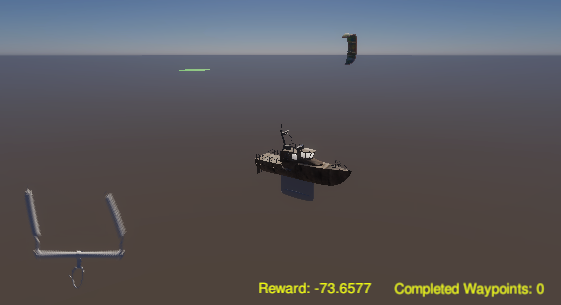
\includegraphics[width=0.8\textwidth]{Images/hard_lock.png}
    \caption{The agent steering on hard lock}\label{hard_lock}
\end{figure}


\subsection{Human Comparison}
Earlier it was mentioned that a heuristic playable game was created to make sure the model felt sensible and could be played by a human player. To create a baseline for the agent's performance 5 human players were asked to play the game for 5 minutes each in heuristic mode and their results were logged. The top 5 performing agents were then run for the same time and the same metrics recorded. 




\subsection{Hardware}\label{sec:hardware_evaluation}
There were several limitations that affected the quality of the training and thus the trained model. First and foremost was compute, as expected when conducting any machine learning training, the more compute available the better. The local machine used for training was a 16-core i9 with 32GB of RAM and a T2000 nvidia graphics, and took approximately 2 hours per million steps completed. This was not a viable option for training the agent to a high level of performance, and so the training was attempted to the university HPC. The HPC has 525 Lenovo nx360 m5 nodes each with two 14 core 2.4 GHz CPUs, and 32 GPU nodes with two cards each. At face value this looks wonderful and training should be a breeze, this was not quite the case. Unity does not support native multi threading, due to the complex nature of its physics engine, so it runs on a single CPU unless manually specified. Manual threading was possible but only for separate tasks that could be called independently of the model, such as the collision detection algorithm. As expected this severely limits the speed of training, and using the hpc did not change these run times.
However, the HPC was not without its advantages, the main being that it was possible to run multiple training runs in parallel, and so the hyperparameter tuning was conducted on the HPC. This would not have been possible on the local machine as it would have taken far too long to test all the combinations. The ability to submit a large batch of jobs to be run in parallel and then the results collection automated was a huge time saver. The HPC also had the advantage of being able to run the training for longer periods of time without causing inconvenience, so even though the training speed was limited it was not a problem to let them run for many days. 

The wait time for resources to be allocated increased the longer the job was scheduled to take 


Thus this project wouldn't have been possible without the HPC.

% The second more major problem was the wait time of the HPC, the longer a job was scheduled the longer it took for the resources to be allocated, for a job that was scheduled for 48 hours on a single node it could take up to 5 days for the job to begin. This was a major problem as it meant that the training could not be conducted in a timely manner, and iteration was very slow. The limited GPU's had the same problem, with only 32 available, and the fact that the HPC was shared with the entire university, it was very difficult to get access to the resources. For this reason the vast majority of training was conducted on the local machine, which had the advantage of also being able to see the training in real time, albeit slowly.   


\section{Critical Evaluation}


\subsection{Objective's Met}
Table opf objectives and outcome goals and wheather they were met or not



